\newgeometry{top=1cm}
\subsection{User Info Screen}
The user info screen is the last that users can access through the tab selector. It shows the profile image of the user at the top, with his/her nickname and email. Below the screen is divided in two main subsections:
\begin{itemize}
    \item Account: it contains two buttons, "change name" and "delete account", that gives to the users the possibility to change their display name and delete their account.
    \item Family: this subsection manage the synchronization with family members, and contains 4 buttons: "share family" that give to the users the possibility to generate a qr code and give to the other users the possibility to join their family; "leave family", once pressed, pop up an alert dialogue to ask users if they really want to leave the family group (whether they're a part of it); "family members" open a new screen and shows the list of users of a family; "join family" pop up a dialog where users have the possibility to join a family group by scanning a qr code or inserting manually the id of a family group.
\end{itemize}

Finally at the bottom there are some other buttons and finally the log out button.

\vspace*{-0.3cm}
\begin{figure}[H]
  \begin{minipage}{0.5\textwidth}
  \centering
    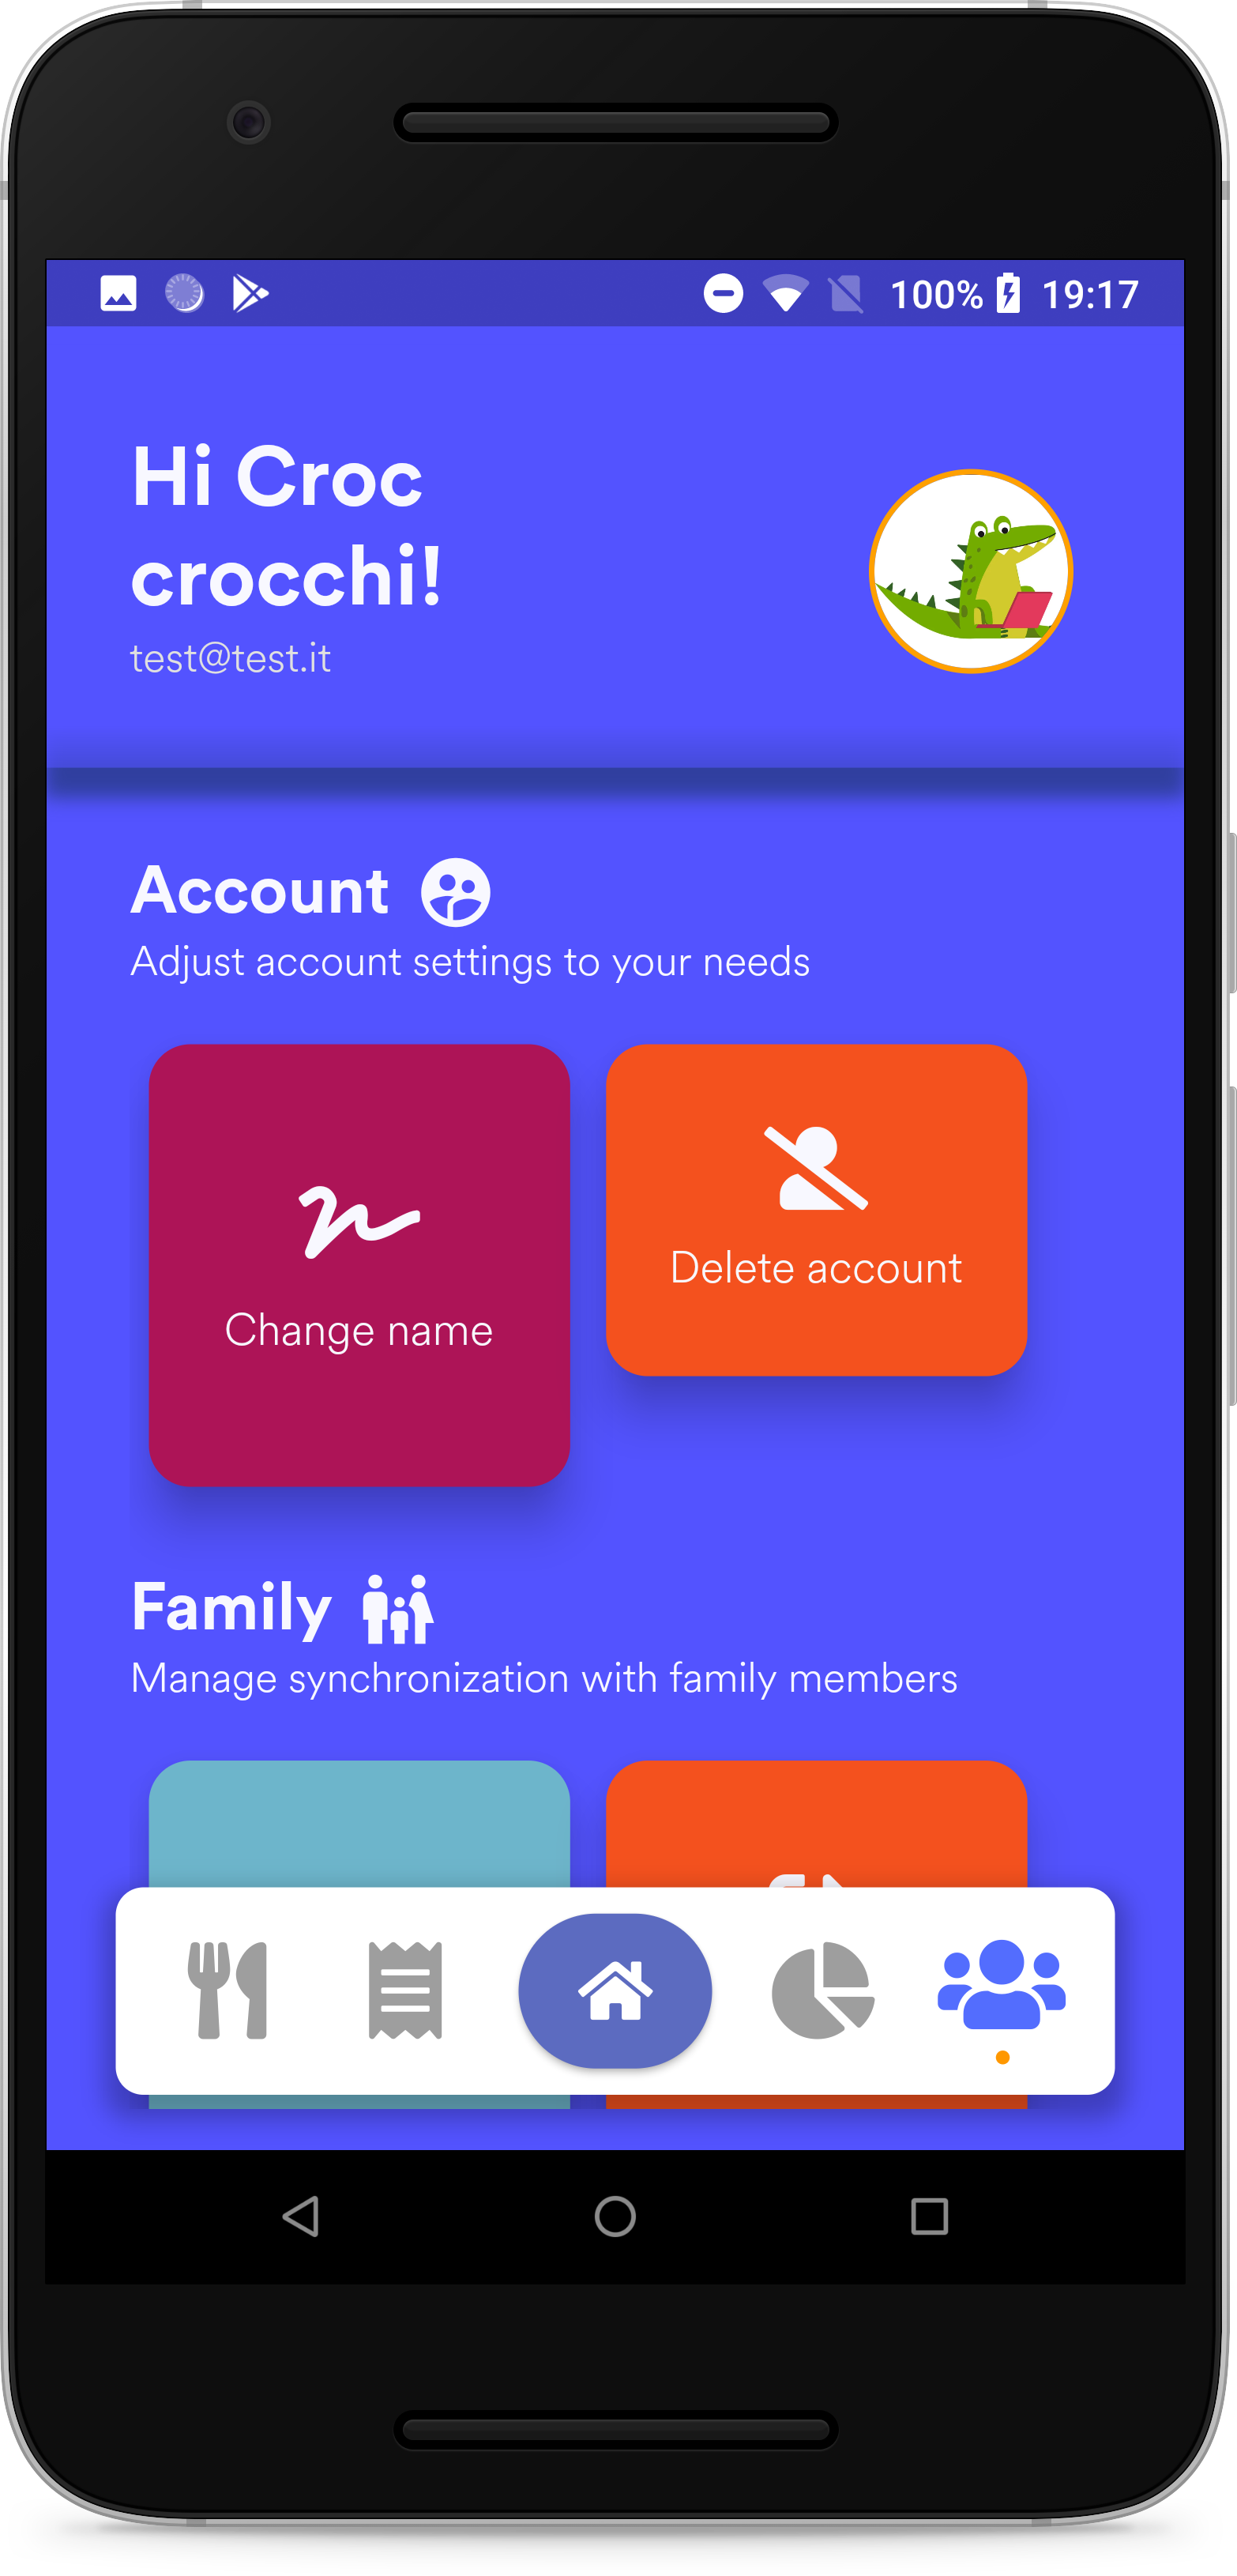
\includegraphics[width=42.mm,scale=0.9]{./Images//Mobile_mocks/user1.png}
    \vspace*{-0.3cm}
    \caption{Mobile user info screen 1}
    \end{minipage}
\hfill
   \begin{minipage}{0.5\textwidth}
     \centering
     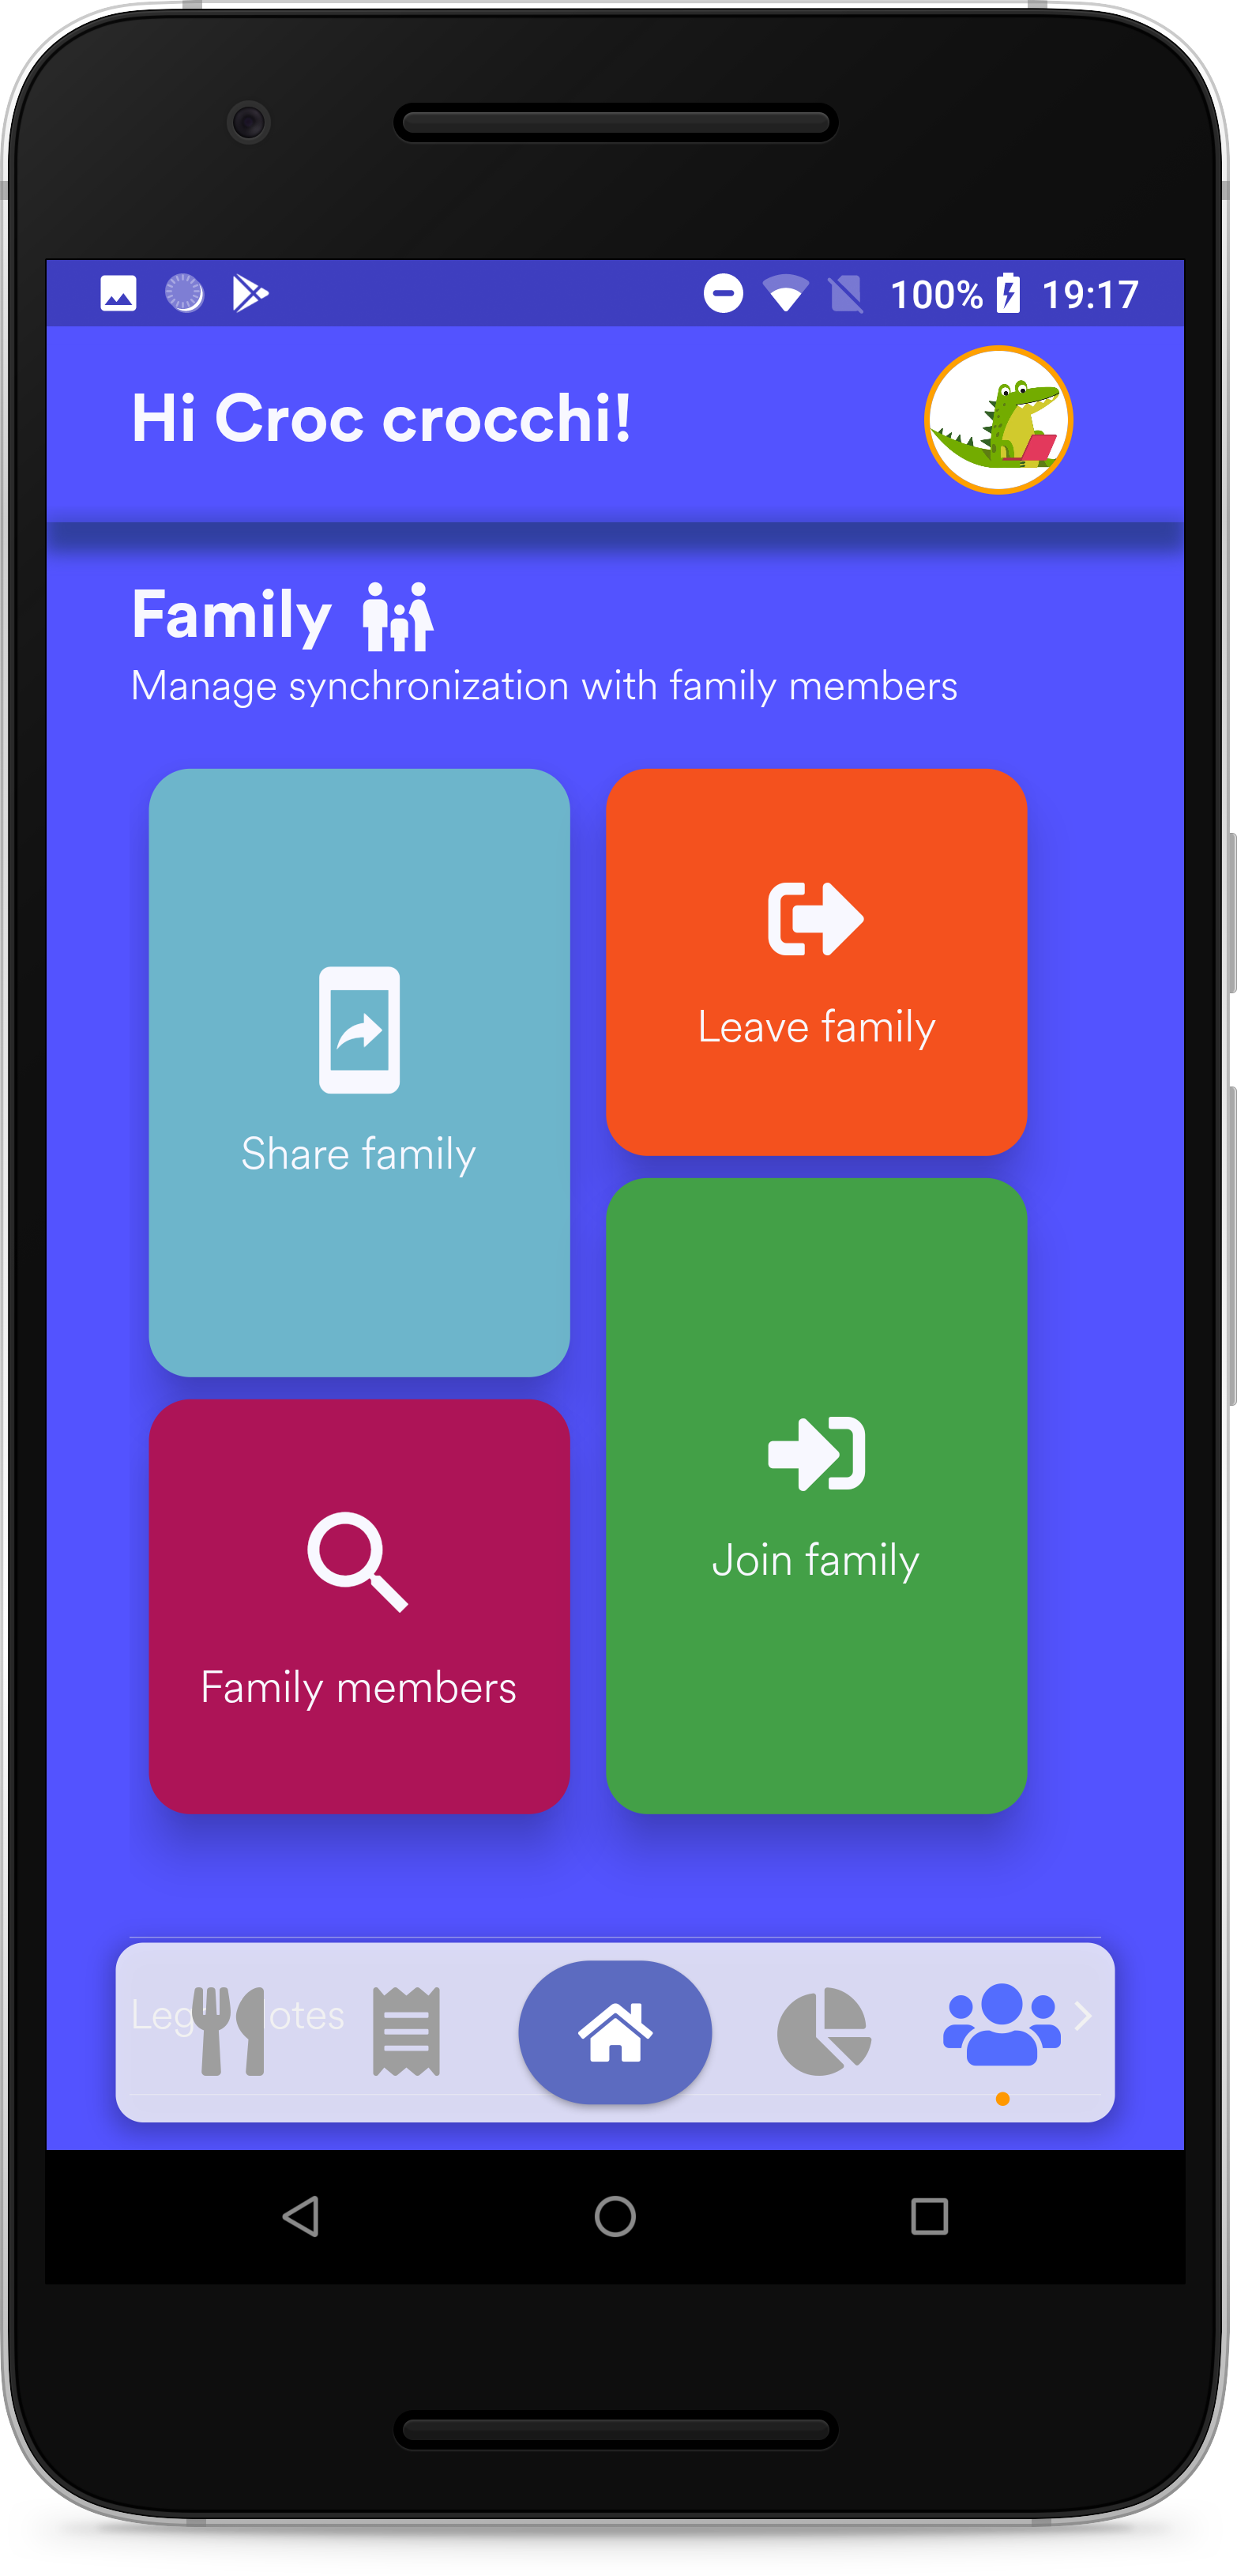
\includegraphics[width=42mm,scale=0.9]{./Images//Mobile_mocks/user2.png}
     \vspace*{-0.3cm}
     \caption{Mobile user info screen 2}
   \end{minipage}
\end{figure}

\vspace*{-0.3cm}
\begin{figure}[H]
  \centering
    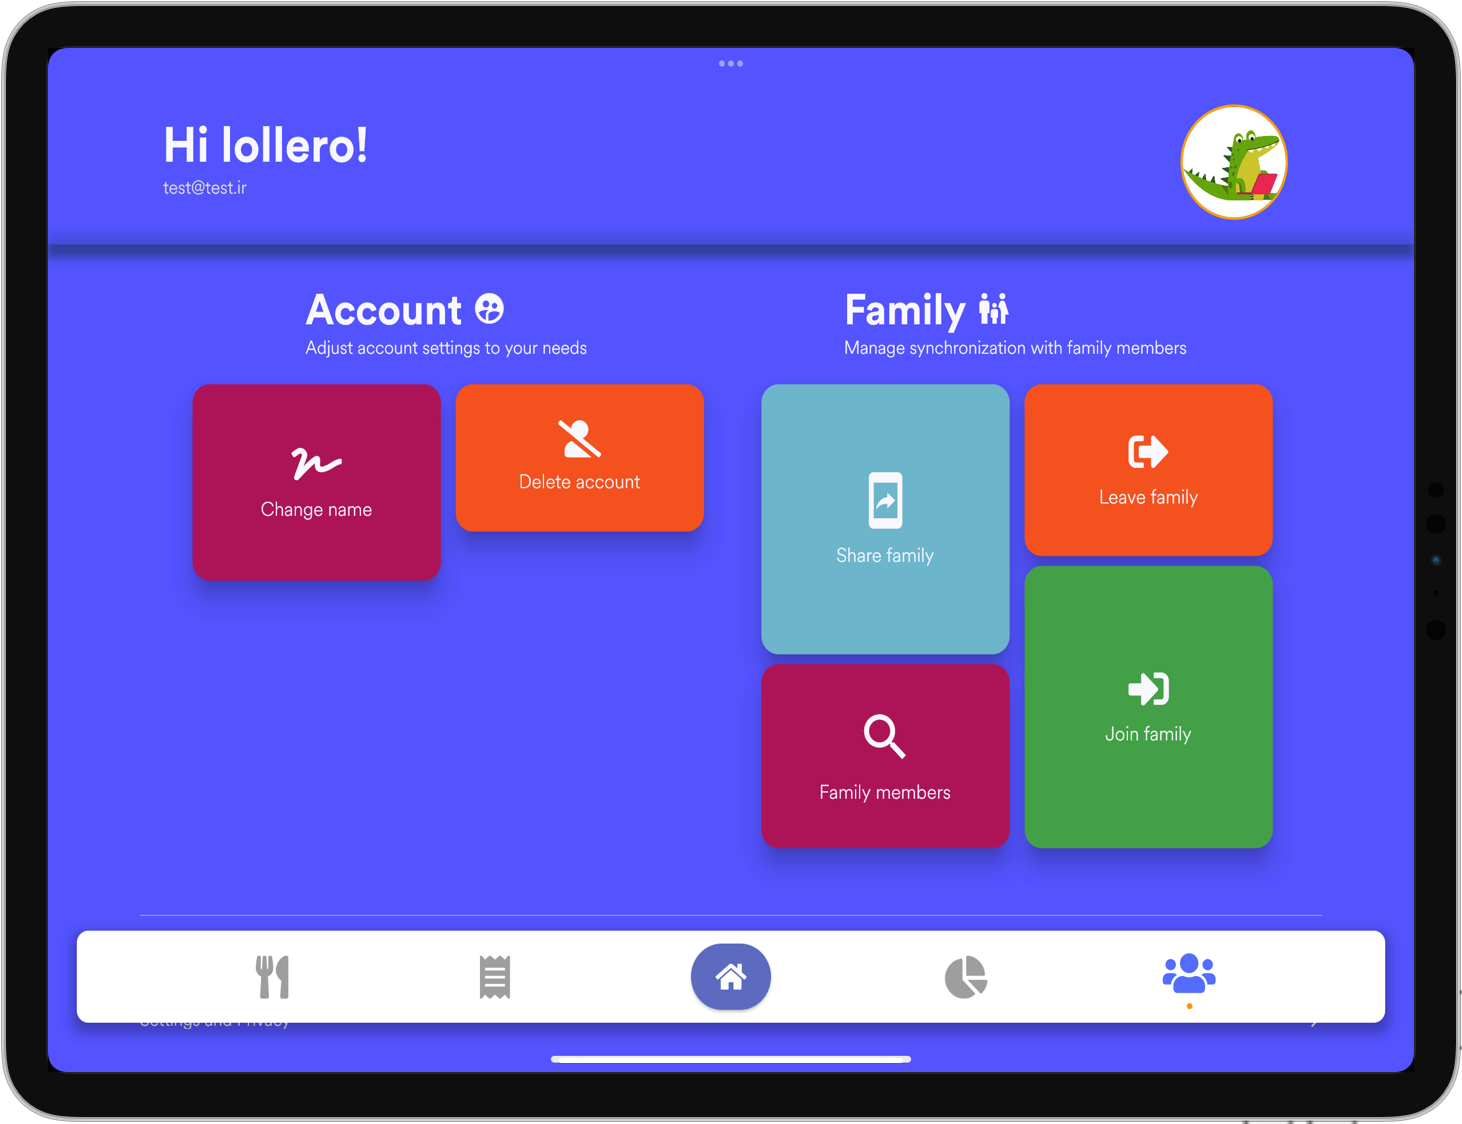
\includegraphics[scale=0.22]{./Images//Tablet_mocks/user1.png}
    \vspace*{-0.3cm}
    \caption{Tablet user info screen}
\end{figure}